%%%%%%%%%%%%%%%%%%%%%%%%%%%%%%%%%%%%%%%%%%%%%%%%%%%%%%%%%%%%%%%%%%%%%%%%%%%%
%  第14回 例題1〜4（原本 20161215143926.pdf の p64/p65/p67/p68 より）
%  原本は「問題枠 →(指針)空欄→【KEY】」で解答が載っていないため，
%  【指針】と【解答】は本文の説明・練習問題の解答の解き方に合わせて書き起こした．
%  ※ このファイルは記録用。実体は physics_ch14.tex に流し込み済み。
%%%%%%%%%%%%%%%%%%%%%%%%%%%%%%%%%%%%%%%%%%%%%%%%%%%%%%%%%%%%%%%%%%%%%%%%%%%%

%%%%%%%%%%%%%%%%%%%%  例題1（14.1 の直後）  %%%%%%%%%%%%%%%%%%%%
\begin{reidai}{気体に関する各量}
\begin{zuright}{42mm}
\hspace{1zw}気体などに関する以下の各設問に答えよ．ただし重力加速度の大きさを$g\U{m/s^2}$，アボガドロ数を$N_{\mathrm{A}}=6.02\times 10^{23}$，窒素の分子量を28とする．
\begin{komon}
\ko{1} 断面積が$S\U{m^2}$のシリンダーに質量$m\U{kg}$のピストンを入れ，中に気体を封入したところ，ピストンは図の位置で静止した．大気圧を$P_0\U{Pa}$とすると，このとき封入されている気体の圧力はどれだけか．また，シリンダーの底面が気体から受ける力を求めよ．
\ko{2} 窒素$\mathrm{N_2}$気体$56\U{g}$中に含まれる窒素分子の数を求めよ．
\ko{3} 窒素の沸点は$77\U{K}$である．これはセルシウス温度では何度に相当するか．
\ko{4} 水の密度を$\rho\U{kg/m^3}$，大気圧を$P_0\U{Pa}$とする．水深$h\U{m}$の位置における水圧$p(h)\U{Pa}$を右図の水柱の力のつり合いから求めよ．
\end{komon}
\zusep
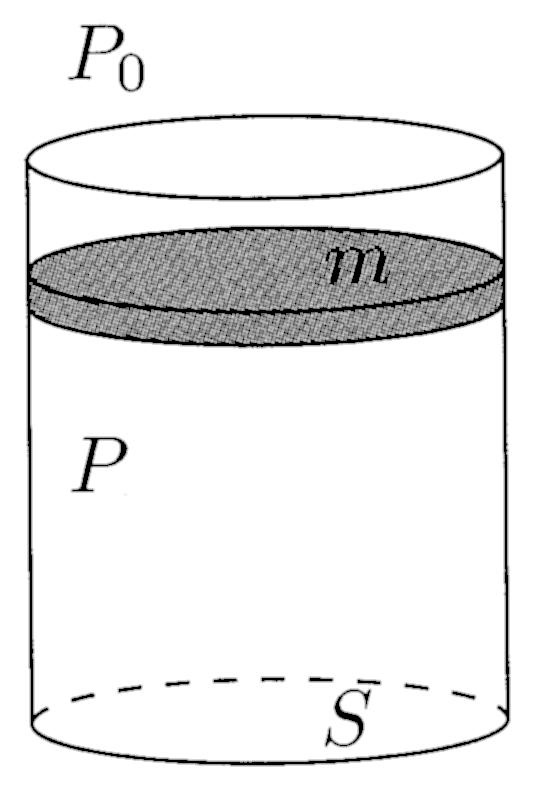
\includegraphics[keepaspectratio,width=26mm]{fig/ch14_ex1_cyl.png}\\[4mm]
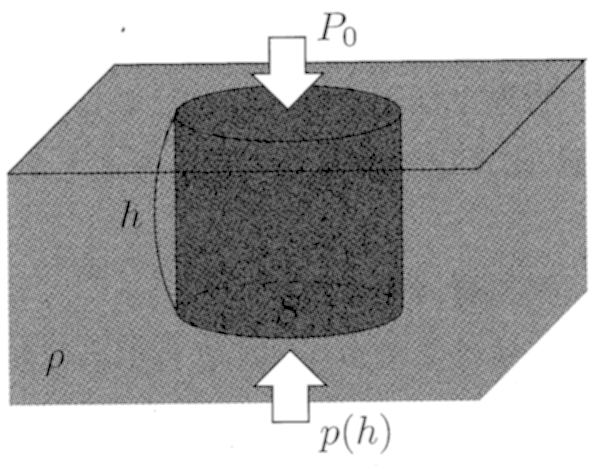
\includegraphics[keepaspectratio,width=42mm]{fig/ch14_ex1_water.png}
\end{zuright}
\end{reidai}

\begin{sisinE}
(1)は，ピストンにはたらく力のつり合いから中の気体の圧力を求める．気体の圧力を問われたら，その気体が押している面についての力のつり合いを考えるのであった．(4)も全く同じ考え方で，図の水柱についての力のつり合いを立てればよい．

(2)は分子量と物質量の関係，(3)は絶対温度とセルシウス温度の関係を使うだけである．
\end{sisinE}

\begin{key}
\hspace{3mm} 圧力$P$[Pa]\hspace{14mm} 単位面積あたりの力で，$F=PS$が成立．\\
\hspace{3mm} 物質量$n$[mol]\hspace{10mm} 分子数$N=nN_A$\hspace{10mm} アボガドロ数$N_A$\\
\hspace{3mm} 絶対温度$T$[K]\hspace{10mm} $T=$セルシウス温度$t\Cel$$+273.15$\\
\hspace{4mm}分子量$M$\hspace{16mm} 分子1[mol]あたりの質量
\end{key}

\begin{kaitou}
\begin{komon}
\ko{1} ピストンにはたらく力のつり合いより，
       \[PS=P_0S+mg\]
       よって，封入されている気体の圧力は，
       \[P=P_0+\frac{mg}{S}\U{Pa}\Ans\]
       また，シリンダーの底面が気体から受ける力は，$F=PS$より，
       \[F=P_0S+mg\U{N}\Ans\]
\ko{2} 窒素の分子量が28であるから，$\mathrm{N_2}$は1[mol]あたり$28\U{g}$である．よって$56\U{g}$の物質量は，
       \[n=\frac{56}{28}=2.0\U{mol}\]
       したがって分子数は，
       \[N=nN_{\mathrm{A}}=2.0\times 6.02\times 10^{23}\]
       \hspace*{2zw}$\fallingdotseq 1.2\times 10^{24}$\,[個]\Ans
\ko{3} $T=t+273.15$より，
       \[t=77-273.15=-196.15\fallingdotseq -196\Cel\Ans\]
\ko{4} 図の水柱（断面積$S\U{m^2}$，高さ$h\U{m}$）にはたらく力は，上面を押す大気からの力$P_0S\U{N}$，水柱自身の重力$\rho hSg\U{N}$，下面を押し上げる力$p(h)S\U{N}$である．水柱は静止しているのでこれらがつり合い，
       \[p(h)S=P_0S+\rho hSg\]
       よって，
       \[p(h)=P_0+\rho gh\U{Pa}\Ans\]
\end{komon}
\end{kaitou}

%%%%%%%%%%%%%%%%%%%%  例題2（14.2 の直後）  %%%%%%%%%%%%%%%%%%%%
\begin{reidai}{状態方程式}
\begin{zuright}{42mm}
\hspace{1zw}容積$V_{\mathrm{A}}$, $V_{\mathrm{B}}\U{m^3}$の容器$\mathrm{A}$，$\mathrm{B}$が，図のようにコックを持つ細い管でつながっている．最初コックは閉じられており，温度$T\U{K}$の理想気体を$\mathrm{A}$，$\mathrm{B}$それぞれに圧力が$P_{\mathrm{A}}$, $P_{\mathrm{B}}\U{Pa}$となるだけ封入した．細管の部分の体積および容器の熱膨張は無視し，気体定数を$R\U{J/mol\cdot K}$として以下の問に答えよ．
\begin{komon}
\ko{1} $\mathrm{A}$，$\mathrm{B}$それぞれの中に含まれる理想気体の物質量$n_{\mathrm{A}}$, $n_{\mathrm{B}}\U{mol}$をそれぞれ求めよ．
\ko{2} 次に，温度を$T\U{K}$に保ったままコックを開いた．このときの容器内の圧力$P\U{Pa}$を求めよ．
\ko{3} (2)において，$\mathrm{A}$から$\mathrm{B}$へ移動した理想気体の物質量$\Delta n\U{mol}$を求めよ．
\ko{4} コックを開いたままの状態で，$\mathrm{A}$の温度を$T_{\mathrm{A}}\U{K}$，$\mathrm{B}$の温度を$T_{\mathrm{B}}\U{K}$に保った．このときの容器の圧力$P'\U{Pa}$を求めよ．
\end{komon}
\zusep
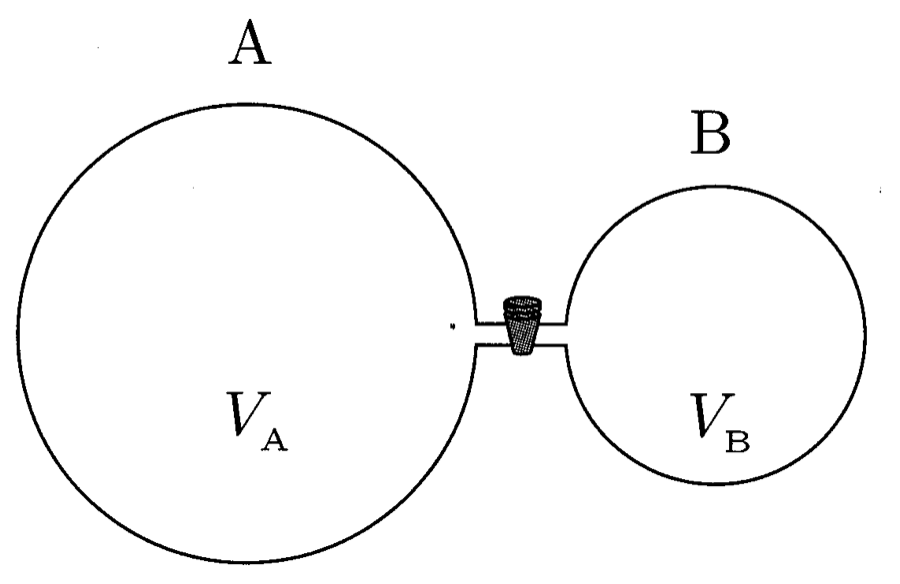
\includegraphics[keepaspectratio,width=42mm]{fig/ch14_ex2_cock.png}
\end{zuright}
\end{reidai}

\begin{sisinE}
コックを開く前と後のそれぞれについて状態方程式を立て，組み合わせればよい．コックを開いたあとは$\mathrm{A}$と$\mathrm{B}$の気体の圧力が等しくなること，そして$\mathrm{A}$，$\mathrm{B}$を合わせた全体の物質量が変わらないことがカギである．

(2)は$\mathrm{A}$と$\mathrm{B}$の温度が同じなので，$\mathrm{A}+\mathrm{B}$を体積$V_{\mathrm{A}}+V_{\mathrm{B}}$の一つの容器とみなしてよい．一方(4)では$\mathrm{A}$と$\mathrm{B}$の温度が違うのでひとまとめにできない．容器ごとに状態方程式を立て，物質量の和が変わらないことを使う．
\end{sisinE}

\begin{key}
\hspace{3mm} 状態方程式\hspace{8mm}$PV=nRT$
\end{key}

\hspace{1zw}左右に圧力差があると気体が流れる．すなわち{\bf 気体が流れていないとき左右の圧力は同じ}である．

\begin{kaitou}
\begin{komon}
\ko{1} コックを開く前の$\mathrm{A}$，$\mathrm{B}$について状態方程式を立てると，
       \[\mathrm{A}:P_{\mathrm{A}}V_{\mathrm{A}}=n_{\mathrm{A}}RT\Eq{1}\]
       \[\mathrm{B}:P_{\mathrm{B}}V_{\mathrm{B}}=n_{\mathrm{B}}RT\Eq{2}\]
       よって，
       \[n_{\mathrm{A}}=\frac{P_{\mathrm{A}}V_{\mathrm{A}}}{RT}\U{mol}, \quad n_{\mathrm{B}}=\frac{P_{\mathrm{B}}V_{\mathrm{B}}}{RT}\U{mol}\Ans\]
\ko{2} コックを開くと$\mathrm{A}$と$\mathrm{B}$の気体の圧力は等しくなる．また，全体の物質量は$n_{\mathrm{A}}+n_{\mathrm{B}}$のまま変わらず，温度も$T$のままである．よって$\mathrm{A}+\mathrm{B}$を体積$V_{\mathrm{A}}+V_{\mathrm{B}}$の一つの容器とみなして状態方程式を立てると，
       \[P(V_{\mathrm{A}}+V_{\mathrm{B}})=(n_{\mathrm{A}}+n_{\mathrm{B}})RT\]
       \MARU{1}\MARU{2}を代入して，
       \[P=\frac{P_{\mathrm{A}}V_{\mathrm{A}}+P_{\mathrm{B}}V_{\mathrm{B}}}{V_{\mathrm{A}}+V_{\mathrm{B}}}\U{Pa}\Ans\Eq{3}\]
\ko{3} コックを開いた後の$\mathrm{A}$内の物質量を$n_{\mathrm{A}}'\U{mol}$とすると，$\mathrm{A}$についての状態方程式より，
       \[PV_{\mathrm{A}}=n_{\mathrm{A}}'RT\]
       $\mathrm{A}$から$\mathrm{B}$へ移動した物質量は$\Delta n=n_{\mathrm{A}}-n_{\mathrm{A}}'$であるから，\MARU{1}\MARU{3}より，
       \[\Delta n=\frac{(P_{\mathrm{A}}-P)V_{\mathrm{A}}}{RT}=\frac{V_{\mathrm{A}}V_{\mathrm{B}}(P_{\mathrm{A}}-P_{\mathrm{B}})}{RT(V_{\mathrm{A}}+V_{\mathrm{B}})}\U{mol}\]
       \hspace*{\fill}\Ans
\ko{4} $\mathrm{A}$と$\mathrm{B}$は細管でつながれているので圧力は等しく$P'\U{Pa}$である．一方，温度は$\mathrm{A}$が$T_{\mathrm{A}}$，$\mathrm{B}$が$T_{\mathrm{B}}$と異なるので，それぞれについて状態方程式を立てる．このときの$\mathrm{A}$，$\mathrm{B}$内の物質量を$n_{\mathrm{A}}''$, $n_{\mathrm{B}}''\U{mol}$とすると，
       \[\mathrm{A}:P'V_{\mathrm{A}}=n_{\mathrm{A}}''RT_{\mathrm{A}}\]
       \[\mathrm{B}:P'V_{\mathrm{B}}=n_{\mathrm{B}}''RT_{\mathrm{B}}\]
       \hspace{1zw}全体の物質量は変わらないので，
       \[n_{\mathrm{A}}''+n_{\mathrm{B}}''=n_{\mathrm{A}}+n_{\mathrm{B}}\]
       すなわち\MARU{1}\MARU{2}より，
       \[\frac{P'V_{\mathrm{A}}}{RT_{\mathrm{A}}}+\frac{P'V_{\mathrm{B}}}{RT_{\mathrm{B}}}=\frac{P_{\mathrm{A}}V_{\mathrm{A}}+P_{\mathrm{B}}V_{\mathrm{B}}}{RT}\]
       よって，
       \[P'=\frac{(P_{\mathrm{A}}V_{\mathrm{A}}+P_{\mathrm{B}}V_{\mathrm{B}})T_{\mathrm{A}}T_{\mathrm{B}}}{T(V_{\mathrm{A}}T_{\mathrm{B}}+V_{\mathrm{B}}T_{\mathrm{A}})}\U{Pa}\Ans\]
\end{komon}
\end{kaitou}

%%%%%%%%%%%%%%%%%%%%  例題3（14.3 の直後）  %%%%%%%%%%%%%%%%%%%%
\begin{reidai}{熱の仕事当量}
\hspace{1zw}質量$500\U{g}$の金属塊を$80\Cel$に熱し，$20\Cel$の水$450\U{g}$の中に入れたところ，全体の温度は$30\Cel$となった．容器の熱容量が$50\U{cal/K}$であるとき，この金属の比熱を求めよ．
\end{reidai}

\begin{sisinE}
熱量の保存を使う．金属塊が失った熱量が，水と容器の温度上昇に使われている．{\bf 容器も水と一緒に温度が上がっている}ことを忘れないこと．なお水の比熱は$1\U{cal/g\cdot K}$である．
\end{sisinE}

\begin{key}
\hspace{3mm} $Q=mc\Delta T$\hspace{2mm}[cal]\hspace{10mm} $Q=C\Delta T$\hspace{2mm}[cal]
\end{key}

\begin{kaitou}
\hspace{1zw}金属の比熱を$c\U{cal/g\cdot K}$とする．金属塊は$80\Cel$から$30\Cel$まで$50\U{K}$下がり，水と容器はともに$20\Cel$から$30\Cel$まで$10\U{K}$上がる．よって，金属塊が失った熱量$Q\U{cal}$，水が得た熱量$Q'\U{cal}$，容器が得た熱量$Q''\U{cal}$はそれぞれ，
\[Q=500\cdot c\cdot(80-30)=25000c\]
\[Q'=450\cdot 1\cdot(30-20)=4500\]
\[Q''=50\cdot(30-20)=500\]
\hspace{1zw}熱量の保存より，金属塊が失った熱量が水と容器の温度上昇に使われたので，
\[Q=Q'+Q''\]
すなわち，
\[25000c=4500+500=5000\]
よって，
\[c=0.20\U{cal/g\cdot K}\Ans\]
\end{kaitou}

%%%%%%%%%%%%%%%%%%%%  例題4（14.4 の直後）  %%%%%%%%%%%%%%%%%%%%
\begin{reidai}{熱力学第一法則}
\begin{komon}
\ko{1} 物体が外界に放出した熱量$q\U{J}$，物体が外界からされた仕事$W\U{J}$，物体の内部エネルギー増加$\Delta U\U{J}$の間に成り立つ熱力学第一法則の式を示せ．
\ko{2} 物体が外界に放出した熱量$q\U{J}$，物体が外界に対してした仕事$w\U{J}$，物体の内部エネルギー増加$\Delta U\U{J}$の間に成り立つ熱力学第一法則の式を示せ．
\end{komon}
\end{reidai}

\begin{sisinE}
与えられている熱量・仕事の向きが，公式の$Q_{in}$（外部が気体に与えた熱量）・$W_{out}$（気体が外部にした仕事）と逆になっている．公式にそのまま代入せず，まず$Q_{in}$と$W_{out}$に読み替えてから代入する，という手順を守ればよい．
\end{sisinE}

\begin{key}
\hspace{3mm} 熱量・仕事の出入りを把握 $\Rightarrow$ 熱力学第一法則の利用
\end{key}

\begin{kaitou}
\begin{komon}
\ko{1} 物体が外界に$q\U{J}$の熱量を放出したのだから，外部が物体に与えた熱量は$Q_{in}=-q\U{J}$である．また，物体が外界からされた仕事が$W\U{J}$なのだから，物体が外界にした仕事は$W_{out}=-W\U{J}$である．これらを$Q_{in}=\Delta U+W_{out}$に代入して，
       \[-q=\Delta U+(-W)\]
       よって，
       \[\Delta U=-q+W\U{J}\Ans\]
\ko{2} (1)と同様に$Q_{in}=-q\U{J}$である．今度は物体が外界にした仕事が$w\U{J}$なのだから，$W_{out}=w\U{J}$である．よって，
       \[-q=\Delta U+w\]
       すなわち，
       \[\Delta U=-q-w\U{J}\Ans\]
\end{komon}
\end{kaitou}
